\documentclass[11pt]{aghdpl}
% Lista wszystkich języków stanowiących języki pozycji bibliograficznych użytych w pracy.
% (Zgodnie z zasadami tworzenia bibliografii każda pozycja powinna zostać utworzona zgodnie z zasadami języka, w którym dana publikacja została napisana.)
\usepackage[english,polish]{babel}

% Użyj polskiego łamania wyrazów (zamiast domyślnego angielskiego).
\usepackage{polski}
\usepackage[utf8]{inputenc}

% dodatkowe pakiety
\usepackage{mathtools}
\usepackage{amsfonts}
\usepackage{amsmath}
\usepackage{amsthm}

% --- < bibliografia > ---

\usepackage[
style=numeric,
sorting=none,
%
% Zastosuj styl wpisu bibliograficznego właściwy językowi publikacji.
language=autobib,
autolang=other,
% Zapisuj datę dostępu do strony WWW w formacie RRRR-MM-DD.
urldate=iso8601,
% Nie dodawaj numerów stron, na których występuje cytowanie.
backref=false,
% Podawaj ISBN.
isbn=true,
% Nie podawaj URL-i, o ile nie jest to konieczne.
url=false,
%
% Ustawienia związane z polskimi normami dla bibliografii.
maxbibnames=3,
% Jeżeli używamy BibTeXa:
backend=biber
]{biblatex}

\usepackage{csquotes}
% Ponieważ `csquotes` nie posiada polskiego stylu, można skorzystać z mocno zbliżonego stylu chorwackiego.
\DeclareQuoteAlias{croatian}{polish}

\addbibresource{cos.bib}


% Nie wyświetlaj wybranych pól.
%\AtEveryBibitem{\clearfield{note}}


% ------------------------
% --- < listingi > ---

% Użyj czcionki kroju Courier.
\usepackage{courier}

\usepackage{listings}
\lstloadlanguages{TeX}

\lstset{
	literate={ą}{{\k{a}}}1
           {ć}{{\'c}}1
           {ę}{{\k{e}}}1
           {ó}{{\'o}}1
           {ń}{{\'n}}1
           {ł}{{\l{}}}1
           {ś}{{\'s}}1
           {ź}{{\'z}}1
           {ż}{{\.z}}1
           {Ą}{{\k{A}}}1
           {Ć}{{\'C}}1
           {Ę}{{\k{E}}}1
           {Ó}{{\'O}}1
           {Ń}{{\'N}}1
           {Ł}{{\L{}}}1
           {Ś}{{\'S}}1
           {Ź}{{\'Z}}1
           {Ż}{{\.Z}}1,
	basicstyle=\footnotesize\ttfamily,
}

% ------------------------

\AtBeginDocument{
	\renewcommand{\tablename}{Tabela}
	\renewcommand{\figurename}{Rys.}
}

% ------------------------
% --- < tabele > ---

\usepackage{array}
\usepackage{tabularx}
\usepackage{multirow}
\usepackage{booktabs}
\usepackage{makecell}
\usepackage[flushleft]{threeparttable}
\usepackage{graphicx}

\graphicspath{ {./images/} }

% defines the X column to use m (\parbox[c]) instead of p (`parbox[t]`)
\newcolumntype{C}[1]{>{\hsize=#1\hsize\centering\arraybackslash}X}

\author{Karol Kaim}
\shortauthor{Karol Kaim}
\titlePL{Projekt i wykonanie prototypu elektronicznego układu zmiany przełożeń w rowerze}
\shorttitlePL{Projekt i wykonanie prototypu elektronicznego układu zmiany przełożeń w rowerze}
\titleEN{Design and implementation of a prototype of an electronic gear-shifting unit in a bicycle}
\shorttitleEN{Design and implementation of a prototype of an electronic gear-shifting unit in a bicycle}
\thesistype{Praca dyplomowa magisterska}
\supervisor{dr inż. Maciej Rosół }
\degreeprogramme{Automatyka i Robotyka}
\date{2016}
\department{Katedra Automatyki i Inzynierii Biomedycznej}
\faculty{Wydział Elektrotechniki, Automatyki,\protect\\[-1mm] Informatyki i Inżynierii Biomedycznej}

\acknowledgements{Serdecznie dziękuję \dots tu ciąg dalszych podziękowań np. dla promotora, żony, sąsiada itp.}


\setlength{\cftsecnumwidth}{10mm}

%---------------------------------------------------------------------------
\setcounter{secnumdepth}{4}
\brokenpenalty=10000\relax

\begin{document}

\titlepages
% Ponowne zdefiniowanie stylu `plain`, aby usunąć numer strony z pierwszej strony spisu treści i poszczególnych rozdziałów.
\fancypagestyle{plain}
{
	% Usuń nagłówek i stopkę
	\fancyhf{}
	% Usuń linie.
	\renewcommand{\headrulewidth}{0pt}
	\renewcommand{\footrulewidth}{0pt}
}

\setcounter{tocdepth}{2}
\tableofcontents
\clearpage

\chapter{Wstęp}
\label{cha:Wstęp}

\section{Wprowadzenie}
\label{sec:Wprowadzenie}
Nowoczesnie technologie znajdują coraz większe zastosowanie w codziennym życiu. Szybki rozwój techniki, miniaturyzacja oraz niższe koszty produkcji sprawiają, że coraz więcej urządzeń codziennego użytku wyposażonych jest w układy elektroniczne, które skutczenie zwiększają ich możliwości. 

Obserwując rynek rowerowy można zauważyć, iż coraz większy nacisk kładziony jest na rozwój oraz zastosowanie wszelkiego rodzaju podzespołów rowerowych, wykorzystujących układy elektroniczne. Doskonałym przykładem takiego urządzenia, a właściwie zespołu urządzeń stanowiących integralną całość produktu, są elektroniczne układy do zmiany przełożeń w rowerze.

Pierwsze próby wykonania takich układów miały miejsce w latach 90 ubiegłego wieku. Jednak ze względu na wygórowaną cenę, wyższą zawodność niż odpowiedniki mechaniczne, oraz wysoką masę, która zwłaszcza w kolarstwie szosowym jest nie do zaakceptowania, nie odniosły komercyjnego sukcesu. Dopiero w roku 2009 japońska firma Shimano wprowadziła na rynek w pełni funkcjonalny układ DuraAce2(\cite{shimanoHistory}). Grupa ugruntowała swoją pozycję na rynku m.in. poprzez to, że rowery wyposażone w napęd tej grupy wygrały już kilkukrotnie wielkie wyścigi kolarskie, np. TourDeFrance.

\section{Cele pracy}
\label{sec:celePracy}

\subsection{Jakiś tytuł}
\subsubsection{Jakiś tytuł w subsubsection}
\subsection{Jakiś tytuł 2}
\chapter{Zestawienie zagadnień wykorzystanych w pracy}
\label{cha:Zestawienie zagadnień wykorzystanych w pracy}

\section{Mechaniczne układy napędowe}
\subsection{Przekładnie mechaniczne}
Układ napędowy to zestaw urządzeń wykorzystywany do napędzania, w skład którego wchodzi źrodło energii, układy pośredniczące w przekazywaniu energii oraz odbiornik energi. Mianem napędu zazwyczaj określa się urządzenia pośredniczące. Najczęściej wykorzystywanymi źródłami enrgii są silniki a odbirniki energii, których zadaniem jest realizowanie odpowiednich ruchów roboczych, przyjmują różne formy zależne od aplikacji.

Układ mechaniczny wykorzystany do przeniesienia ruchu obrotowego z elementu czynnego na element bierny nazywany jest przekładnią mechaniczną. Oprócz transmisji energii, przekładnie umożliwają również zmianę parametrów ruchu - momentu obrotowego oraz prędkości obrotowej. Przekładnie mechaniczne dzieli się na trzy grupy: cięgnowe, cierne i zębate. Przekładnie cięgnowe, które zostały opisane ze wzgędu na zastosowanie w rowerowych układach napędowych, składają się z conajmniej dwóch kół zębatych, rozsuniętych względem siebie, oraz cięgna opasającego. Ze względu na rodzaj zastosowanego cięgna, wyróżnia się przekładnie pasowe oraz łańcuchowe. Przenoszenie siły z cięgna na koło zębate jest możliwe dzięki zastosowaniu odpowiednich połączeń - połączenia cierne, kształtowe lub stałe przymocowanie cięgna do koła zębatego.

\textcolor{red}{@TODO wrzucić schemat przekładni, dodać jakiś przypis doprzełkadni}

Wielkością charakteryzującą przekładnie jest przełożenie. Wyróżnia się przełożenie geometryczne, kinematyczne oraz dynamiczne. Przełożenie kinematyczne to stosunek prędkości kątowej koła czynnego do prędkości kątowej koła biernego:
\textcolor{red}{@TODO wzorek i=w1/w2}

Przełożenie dynamiczne określa stosunek momentu obrotowego na kole biernym do momentu obrotowego koła czynnego.  

\textcolor{red}{@TODO wzorek i=M2/M1}

Przełożenie przekładni jest parametrem bezwymiarwoym. Ze względu na wartość przełożenia przekładni wyróznia się:
\begin{itemize}
\item
Przekładnie przyspieszające lub tzw. multiplikatory. Przekładnie tego typu zwiększają prędkość kątową koła biernego względem prędkości kątowej koła czynnego przy jednoczesnym zmniejszeniu momentu obrotowego koła biernego względem momentu obrotowego koła czynnego. Przełożenie takiej przekładni jest liczbą z zakresu od 0 do 1.
\item
Przekładnie redukujące lub tzw. reduktory. Przekładnie tego typu działają w sposób odwrotny do przekładni przyspieszających - zmniejszają prędkość kątową koła biernego względem prędkości kątowej koła czynnego oraz zwiększają moment obrotowy koła biernego wzlgędem momentu obrotowego koła czynnego. Przełożenei przekładni redukującej jest zawsze większe od 1.
\end{itemize} 


	  
\subsection{Układ napędowy w rowerze}
W przypadku konwencjonalnego układu napędowego stosowanego w rowerach źródłem energii jest rowerzysta. Siła przyłożona do ramienia korby generuje moment obrotowy, który przenoszony jest, przy pomocy mechanizmu korbowego i łańcucha, na koło zębate na stałe przymocowoane do piasty tylnego koła. Moment obrotowy koła napędzającego powoduje powstanie sił obwodowych, składających się na siłę napędową, która wprawia rower w ruch postępowy.

\section{Urządzenia pomiarowe}
\subsection{Pomiar prędkości kątowej}

Możliwość pomiaru prędkości kątowej jest kluczowa ze względu na wykonanie trybu automatycznej zmiany przełożeń. Na podstawie aktualnej prędkości kątowej tylnego koła wyznaczona zostanie chwilowa prędkość liniowa. Prędkość kątowa jest wielkością wektorową, jednak w rozważaniach dotyczących pracy brana pod uwagę jest jedynie chwilowa wartość prędkości kątowej. Ta zdefiniowana jest jako zmiana drogi kątowej w czasie:
\begin{equation}
\omega = \frac{d\varphi}{dt}
\end{equation}
\begin{eqwhere}[2cm]
	\item[$\varphi$] droga kątowa
	\item[$t$] czas
\end{eqwhere}
Wyznaczenie chwilowej wartości prędkości kątowej wykonane zostało w oparciu o czujniki zbliżeniowy załączany magnetycznie, który został na stałe przymocowany do ramy roweru, w niewielkiej odległości od tylnego koła. Zasada działania takiego czujnika jest analogiczna do działania zwykłego przycisku monostabilnego. Obwód w czujniku jest domyślnie rozwarty. Zwarcie następuje w momencie zbliżenia magnesu do czujnika. Magnes przyczepiony został do szprychy roweru. Taki sam sposób pomiaru prędkości można znaleźć w komercyjnych licznikach rowerowych oferowanych na rynku. Autor zdecydował się na zastosowanie dwóch magnesów w celu zwiększenia dokładności pomiaru. Dysponując pomiarem czasu pomiędzy kolejnymi zwarciami czujnika magnetycznego, które, ze względu na zastosowanie dwóch magnesów, następują w wyniku obrotu koła o kąt $\pi$ , można wyznaczyć chwilową wartość prędkości kątowej: 
\begin{equation}
\omega = \frac{\pi}{T}
\end{equation}
\begin{eqwhere}[2cm]
	\item[$T$] czas od ostatniego zwarcia czujnika magnetycznego
\end{eqwhere}
Chwilowa wartość prędkości liniowej to stosunek przebytej drogi liniowej do czasu:
\begin{equation}
v = \frac{s}{t}
\end{equation}
\begin{eqwhere}[2cm]
	\item[$s$] droga liniowa
	\item[$v$] prędkość liniowa
\end{eqwhere}
 Związek pomiędzy drogą liniową a drogą kątową wyraża się wzorem:
\begin{equation}
\varphi = \frac{s}{r}
\end{equation}
\begin{eqwhere}[2cm]
	\item[$r$] promień okręgu
\end{eqwhere}
W układzie pomiarowym z dwoma magnesami, wartość drogi kątowej w momencie zwarcia czujnika magnetycznego wynosi $\pi$. Biorąc pod uwagę powyższe zależnosci, chwilowa wartość prędkości liniowej poruszającego się roweru może zostać wyznaczona z zależności:
 \begin{equation}
v = \frac{\pi R}{T}
\end{equation}
\begin{eqwhere}[2cm]
	\item[$R$] promień koła rowerowego
\end{eqwhere}
\subsection{Pomiar przyspieszeń}
Z drugiej zasady dynamiki Newtona wynika, iż przyspieszenie jest proporcjonalne do wypadkowej siły działającej na ciało. Znajomość chwilowej wartośći oraz zwrotu przyspieszenia jest drugą istotną informacją, która została wykorzystana przy projektowaniu sterownika trybu automatycznego, gdyż może dostarczyć wiedzy na temat aktualnej dynamiki ruchu.

Pomiar przyspieszenia został zrealizowany w oparciu o zastosowanie akcelerometru wykonanego w technologii MEMS( z ang. {\em Micro Electro-Mechanical Systems}). Układy MEMS to urządzenia wykonane w miniaturowej skali, które integrują ze soba elementy mechaniczne oraz elektroniczne. Wykorzystywane głównie jako czujniki przetwarzające wielkości mechaniczne na wielkości elektryczne. Czujniki wykonane w technologii MEMS posiadają kilka znaczących zalet, które sprawiają, że spektrum zastosowań staje się coraz szersze. Są to m.in. niska cena, niewielkie rozmiary, niskie zużycie energii oraz prosta integracja z układami mikroprocesorowymi.

\subsection{Pomiar kąta nachylenia}

\section{Sterowanie}


\subsection{Zamknięty układ regulacji}
\subsection{Serwomechanizm}

\section{Kondycjonowanie sygnałów}


\subsection{Drganie styków}
\subsection{Filtr donlnoprzepustowy}
\chapter{Zestawienie zagadnień wykorzystanych w trakcie realizacji projektu}
\label{cha:Zestawienie zagadnien wykorzystanych w pracy}

W niniejszym rozdziale przedstawiono zagadnienia wykorzystane do realizacji układu zmiany przełożeń. Zamieszczono opis zasady działania serwomechanizmu, filtru dolnoprzepustowego RC oraz metod pomiarowych wielkości fizycznych, niezbędnych do poprawnego działania sterownika układu.
 
\section{Serwomechanizm - budowa i zasada działania}
Serwomechanizm to układ automatycznej regulacji, który służy do precyzyjnego sterowania silnikiem elektrycznym. Serwomechanizm wykorzystany w pracy pozycjonuje wózek przerzutki w zadanym położeniu.

Układy automatycznej regulacji w serwomechanizmach to zazwyczaj układy zamknięte z ujemną pętlą sprzężenia zwrotnego. Schemat takiego układu regulacji został przedstawiony na rys. \ref{fig:zamknietyUklad}. Zastosowanie ujemnego sprzężenia zwrotnego umożliwia osiągnięcie celu sterowania, pomimo występujących zakłóceń. Mogą to być zakłócenia związane z pomiarami wyjścia, zakłócenia działające na obiekt lub zakłócenia sterowania. Zasada działania układu ze sprzężeniem zwrotnym polega na porównaniu aktualnej wartości wielkości regulowanej $y$ z wartością zadaną $r$, wyznaczeniu wartości uchybu regulacji $e$ i pobudzenia do pracy regulatora, którego akcja redukuje błąd regulacji, pomimo ciągle działających zakłóceń $z$ \cite{zamknietyB}.
\begin{figure}[h]
    \centering
    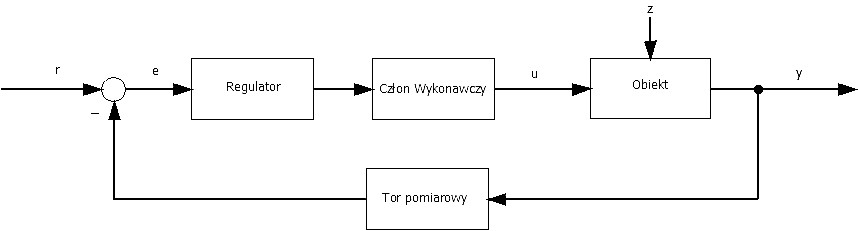
\includegraphics[scale=0.4]{zamknietyUkladRegulacji.jpg}
    \caption{Schemat zamkniętego układu regulacji z ujemną pętlą sprzężenia zwrotnego. Opis sygnałów : $r$ – wartość zadana,  $e$ – uchyb regulacji, $u$ – sterowanie generowane przez regulator , $y$ – wyjście z obiektu, $z$ – zakłócenia działające na obiekt.}
    \label{fig:zamknietyUklad}
\end{figure}

Serwomechanizm zbudowany jest z kilku podstawowych elementów, takich jak silnik elektryczny, układ pomiarowy pozycji/prędkości wału silnika, regulator oraz układ mocy. W serwomechanizmach stosowane są silniki prądu stałego lub przemiennego. Serwomechanizmy oferowane na rynku mogą pracować w kilku trybach:
\begin{itemize}
\item
     Tryb regulacji położenia - układ automatycznej regulacji dąży do osiągnięcia zadanej pozycji wału silnika.
\item
    Tryb regulacji prędkości - układ automatycznej regulacji dąży do osiągnięcia zadanej prędkości obrotowej wału silnika.
\item
    Tryb regulacji momentu obrotowego - układ automatycznej regulacji dąży do osiągnięcia zadanego momentu obrotowego generowanego przez silnik.
\end{itemize}

Szczegóły dotyczące serwomechanizmu, wykorzystanego do realizacji projektu, zostały przedstawione w pkt. \ref{serwo}  
%____________________________________________________________________________________________________________  
\section{Pasywny filtr dolnoprzepustowy RC}

Filtr to układ, który przenosi na wyjście sygnały o określonej częstotliwości. Filtr dolnoprzepustowy przenosi na wyjście sygnały o niskiej częstotliwości, natomiast blokuje sygnały szybkozmienne. Ze względu na konstrukcję filtru, można je podzielić również na filtry pasywne, zbudowane tylko w oparciu o elementy RLC, i aktywne, wykorzystujące dodatkowo np. wzmacniacze operacyjne. 

Najprostszy filtr dolnoprzepustowy to pasywny filtr RC zbudowany z opornika o rezystancji $R$ i kondensatora o pojemności $C$ - rys. \ref{fig:filtrRC1}. 
\begin{figure}[h]
    \centering
    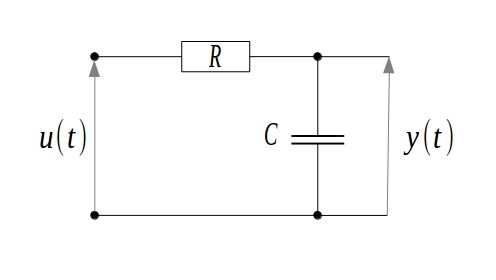
\includegraphics[scale=0.4]{filtrRC.jpg}
    \caption{Pasywny filtr dolnoprzepustowy RC - $u(t)$ sygnał wejściowy filtru, $y(t)$ sygnał wyjściowy filtru.}
    \label{fig:filtrRC1}
\end{figure}


Przyjmując napięcie na kondensatorze jako zmienną stanu $x(t)$, sterowanie układu jako sygnał $u(t)$ a obserwację jako sygnał wyjściowy filtru $y(t)$, oraz pamiętając o tym, że prąd płynący przez obwód jest równy zmianie ładunku na kondensatorze, można zapisać model matematyczny układu w postaci równań stanu:
\begin{equation}
\begin{gathered}
    \dot{x}(t) = -\frac{1}{RC}x(t) + u(t) \\
    y(t) = x(t)
     \label{eq:stanuRC}
\end{gathered}
\end{equation}

Zgodnie z definicją $4.1$ w pkt. \textit{Zagadnienie realizacji transmitancji} w pracy \cite{graba}, transmitancja operatorowa filtru RC jest opisana zależnością:
\begin{equation}
    G(s) = \frac{RCs}{RCs + 1}
    \label{eq:transRc}
\end{equation}

Z powyższego równania wynika, że obwód RC jest  układem inercyjnym I rzędu, którego stała czasowa wynosi:
\begin{equation}
   T = RC
    \label{eq:stalaCzasowaRC}
\end{equation}

Charakterystyka amplitudowa obiektu inercyjnego I rzędu wykazuje zdolność obiektu do tłumienia amplitudy sygnałów o wysokich częstotliwościach, co jest zgodne z zasadą działania filtru dolnoprzepustowego.
\begin{figure}[h]
    \centering
    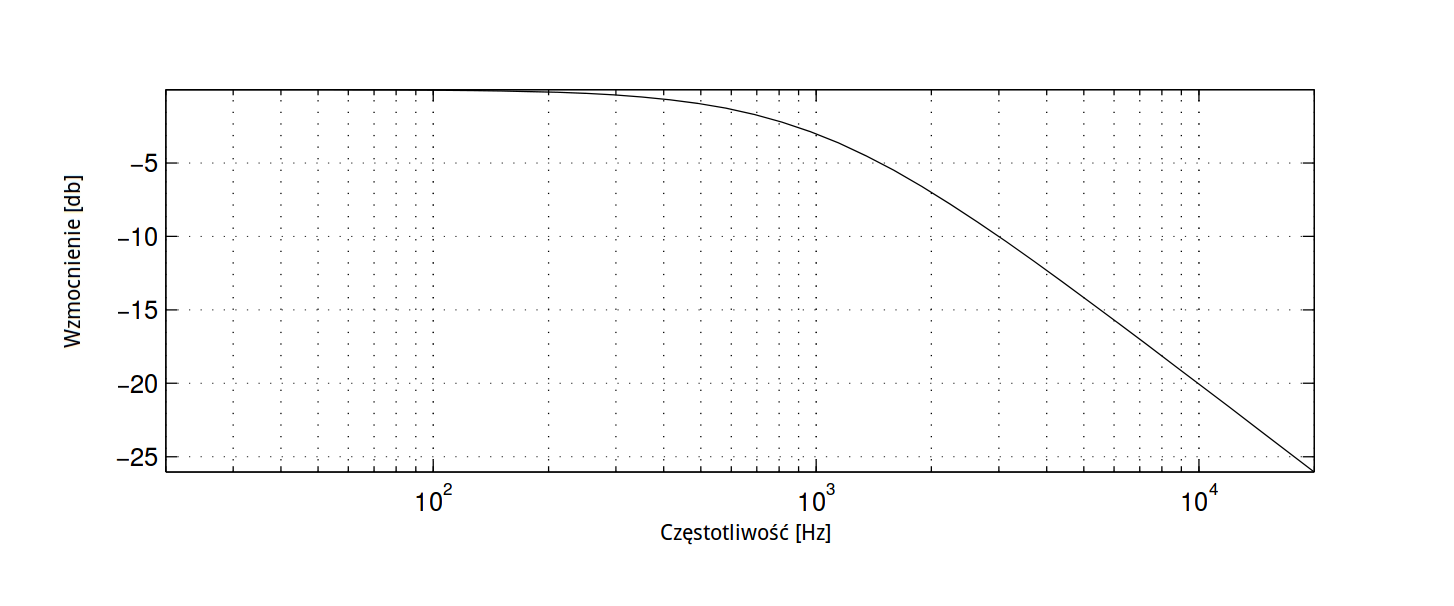
\includegraphics[scale=0.23]{charakterystykaAmp.png}
    \caption{Przykładowa charakterystyka amplitudowa układu inercyjnego I rzędu \cite{charakterystykaAmp}.}
    \label{fig:charamp}
\end{figure}

\label{filtrRc}
%____________________________________________________________________________________________________________  
\section{Metody pomiarowe wielkości fizycznych}
\subsection{Pomiar prędkości kątowych koła i mechanizmu korbowego.}

Możliwość pomiaru prędkości kątowej jest kluczowa ze względu na wykonanie trybu automatycznej zmiany przełożeń. Pomiar prędkości kątowej mechanizmu korbowego umożliwi wyznaczenie aktualnej wartości kadencji.

Prędkość kątowa jest wielkością wektorową, jednak w rozważaniach dotyczących pracy brana pod uwagę jest jedynie chwilowa wartość prędkości kątowej. Ta zdefiniowana jest jako zmiana drogi kątowej w czasie:
\begin{equation}
    \omega = \frac{d\varphi}{dt}
    \label{eq:predkoscKatowa}
\end{equation}
gdzie:
\begin{eqwhere}[2cm]
	\item[$\varphi$] droga kątowa,
	\item[$t$] czas.
\end{eqwhere}
Wyznaczenie chwilowej wartości prędkości kątowej jest możliwe dzięki zastosowaniu czujnika zbliżeniowego załączanego magnetycznie, który jest przymocowany do ramy roweru, w niewielkiej odległości do tylnego koła. Zasada działania takiego czujnika jest analogiczna do działania zwykłego przycisku monostabilnego. Obwód w czujniku jest domyślnie rozwarty. Zwarcie następuje w momencie zbliżenia magnesu do czujnika. Magnes przyczepiony jest do szprychy roweru. Taki sam sposób pomiaru prędkości można znaleźć w komercyjnych licznikach rowerowych oferowanych na rynku. Autor zdecydował się na zastosowanie dwóch magnesów w celu zwiększenia dokładności pomiaru. Dysponując pomiarem czasu pomiędzy kolejnymi zwarciami czujnika magnetycznego, które, ze względu na zastosowanie dwóch magnesów, następują w wyniku obrotu koła o kąt $\pi$ , można wyznaczyć chwilową wartość prędkości kątowej: 
\begin{equation}
    \omega_{wheel} = \frac{\pi}{T_{wheel}}
\end{equation}
gdzie:
\begin{eqwhere}[2cm]
    \item[$\omega_{wheel}$] prędkość kątowa tylnego koła $[\frac{rad}{s}]$,
	\item[$T_{wheel}$] czas pomiędzy kolejnymi zwarciami czujnika magnetycznego koła $[s]$.
\end{eqwhere}
Prędkość kątowa mechanizmu korbowego została wyznaczona w sposób analogiczny. Zbliżeniowy czujnik magnetyczny, na stałe przymocowany do ramy roweru w bliskiej odległości mechanizmu korbowego, jest zwierany w każdym cyklu dzięki zastosowaniu magnesu, który jest przyklejony do ramienia mechanizmu korbowego. Ze względu na zastosowanie jednego magnesu, przyrost drogi kątowej jest dwa razy większy, niż w przypadku pomiaru prędkości kątowej koła roweru i jego wartość wynosi 2$\pi$:
\begin{equation}
    \omega_{crank} = \frac{2\pi}{T_{crank}}
\end{equation}
gdzie:
\begin{eqwhere}[2cm]
    \item[$\omega_{wheel}$] prędkość kątowa mechanizmu korbowego $[\frac{rad}{s}]$,
	\item[$T_{crank}$] czas pomiędzy kolejnymi zwarciami czujnika magnetycznego mechanizmu korbowego $[s]$.
\end{eqwhere}
\subsection{Prędkość liniowa roweru}
Wartość prędkości liniowej to stosunek przebytej drogi do czasu:
\begin{equation}
    v = \frac{s}{t}
\end{equation}
gdzie:
\begin{eqwhere}[2cm]
	\item[$s$] droga liniowa,
	\item[$v$] prędkość liniowa.
\end{eqwhere}
 Związek pomiędzy drogą liniową a drogą kątową, punktu poruszającego się po okręgu o promieniu $r$,wyraża się wzorem:

\begin{equation}
    \varphi = \frac{s}{r}
\end{equation}

W układzie pomiarowym prędkości kątowej koła roweru, który wykorzystuje dwa magnesy, wartość drogi kątowej w momencie zwarcia czujnika magnetycznego wynosi $\pi$. Dysponując pomiarem czasu $T_{wheel}$, chwilowa wartość prędkości liniowej tylnego koła, a zarazem całego roweru, może zostać wyznaczona z zależności:
 \begin{equation}
    \label{eq:zaleznoscNaPredkosc}
    v_{bike} = \frac{\pi R}{T_{wheel}}
\end{equation}
gdzie:
\begin{eqwhere}[2cm]
    \item[$v_{bike}$] prędkość roweru $[\frac{m}{s}]$,
	\item[$R$] promień koła rowerowego $[m]$.
\end{eqwhere}
%____________________________________________________________________________________________________________  
\subsection{Inercyjna jednostka pomiarowa IMU}
Inercyjna jednostka pomiarowa (ang. {\em Inertial Measurement Unit}) to układ składający się z kilku czujników pomiarowych, pozwalających wyznaczyć orientację obiektu w przestrzeni trójwymiarowej. Stosowane m.in. w systemach stabilizacji bezzałogowych statków powietrznych. W realizowanym projekcie wykorzystana zostanie możliwość wyznaczenia kąta nachylenia podłoża, po którym porusza się rower z zamontowaną jednostką pomiarową IMU.

Jednostki IMU zazwyczaj wyposażone są w trzyosiowy akcelerometr, trzyosiowy żyroskop oraz magnetometr. Wszystkie czujniki to urządzenia wykonane w miniaturowej skali oraz technologii MEMS (ang. {\em Micro Electro-Mechanical Systems}), które integrują elementy mechaniczne oraz elektroniczne. Wykorzystywane głównie jako czujniki przetwarzające wielkości mechaniczne na wielkości elektryczne. Czujniki wykonane w technologii MEMS posiadają kilka znaczących zalet, które sprawiają, że spektrum zastosowań staje się coraz szersze. Są to m.in. niska cena, niewielkie rozmiary, niskie zużycie energii oraz prosta integracja z układami mikroprocesorowymi. 

%____________________________________________________________________________________________________________  
\subsubsection{Pomiar przyspieszeń - akcelerometr}
Akcelerometr to urządzenie pomiarowe, które umożliwia pomiar przyspieszenia dynamicznego ciała, na które działa niezerowa siła wypadkowa, oraz przyspieszenia statycznego ciała znajdującego się w ziemskim polu grawitacyjnym. Akcelerometry zazwyczaj działają na zasadzie przetworników pojemnościowych. Pomiar dokonywany jest dzięki zastosowaniu kondensatorów różnicowych, których ruchome okładki wychylane są z położenia równowagi pod wpływem działających sił bezwładności.

Akcelerometry są powszechnie wykorzystywane w różnego rodzaju aplikacjach. Układy sterujące poduszkami powietrznymi, systemy alarmowe w samochodach czy tzw. system ruszania na wzniesieniu to tylko niektóre przykłady z branży motoryzacyjnej \cite{stAkcel}.

Układy do pomiaru przyspieszenia wykonane w technologii MEMS zazwyczaj składają się z trzech akcelerometrów, które umożliwiają pomiar przyspieszenia w trzech różnych kierunkach. Akcelerometr został zamontowany w rowerze w taki sposób, aby kierunek osi \textit{x} był równoległy do podłoża (rys. \ref{fig:rownia}).
%____________________________________________________________________________________________________________  
\subsubsection{Pomiar prędkości kątowych - żyroskop}
Żyroskop to urządzenie pomiarowe dostarczające informacji na temat chwilowej prędkości obrotowej układu pomiarowego. Żyroskopy wykonane w technologii MEMS to czujniki pojemnościowe wykorzystujące efekt Coriolisa. Układ dwóch wibrujących mas, umieszczony na obrotowej tarczy, zmienia swoje położenie względem osi obrotu w zależności od chwilowej prędkości obrotowej. W wyniku zmiany położenia układu mas odkształceniu ulega tarcza, która stanowi okładkę kondensatora. W efekcie następuje różnicowa zmiana pojemności kondensatora, która przetwarzana jest na chwilową prędkość obrotową \cite{stGyro}.

Żyroskop, podobnie jak akcelerometr, to układ trzech czujników pozwalający na pomiar prędkości kątowej w trzech różnych kierunkach. Zamontowany został w taki sposób, aby kierunek osi żyroskopu \textit{x} oraz \textit{z}  był równoległy do podłoża.

%____________________________________________________________________________________________________________  
\section{Estymata kąta nachylenia podłoża}
Kąt nachylenia podłoża, po którym porusza się rower, to ostatnia z wielkości  brana pod uwagę przez algorytm automatycznej zmiany przełożeń. Wielkość ta wyznaczana jest pośrednio, poprzez zastosowanie filtru komplementarnego, wykorzystującego dane pomiarowe pochodzące z akcelerometru oraz żyroskopu.

%____________________________________________________________________________________________________________ 
\subsection{Analiza danych pomiarowych akcelerometru}
\label{pomiaryAkcel}
Przykład zamieszczony na rysunku \ref{fig:rownia} przedstawia ciało znajdujące się na równi pochyłej. Przyspieszenie ziemskie \textit{$g$} zostało rozłożone na kierunki składowe wzdłuż osi pomiarowych akcelerometru - \textit{$a_x$} oraz \textit{$a_y$}. Wektory składowe wraz z przyspieszeniem ziemskim stanowią trójkąt podobny do trójkąta, będącego przekrojem równi pochyłej, o kącie nachylenia oznaczonym jako $\alpha$. Stosunek długości przyprostokątnej leżącej naprzeciw kąta $\alpha$ do wartości drugiej przyprostokątnej, które odpowiadają wartością przyspieszeń mierzonym przez akcelerometr odpowiednio wzdłuż osi $x$ i $y$, wynosi $\tan{\alpha}$. Zastosowanie funkcji odwrotnej pozwala wyznaczyć kąt nachylenia równi:
\begin{equation}
    \alpha=\arctan{\frac{a_x}{a_y}}
    \label{eq:rowniaRadian}
\end{equation}
gdzie:
\begin{eqwhere}[2cm]
	\item[$\alpha$] kąt nachylenia podłoża
	\item[$a_x$] przyspieszenie akcelerometru mierzone wzdłuż osi $X$,
	\item[$a_y$] przyspieszenie akcelerometru mierzone wzdłuż osi $Y$.
\end{eqwhere}
Z zależności (\ref{eq:rowniaRadian}) można wyznaczyć wartość miary łukowej kąta wyrażonej w radianach. W odniesieniu do kąta nachylenia podłoża, po którym porusza się rower, zdecydowanie bardziej intuicyjną jednostką są stopnie. Przekształcenie miary kąta wyrażonej w radianach na miarę kąta wyrażoną w stopniach opisane jest poniższą zależnością:
\begin{equation}
    \alpha_{deg}=\frac{180\alpha}{\pi}
    \label{eq:rowniaStopnie}
\end{equation}
gdzie:
\begin{eqwhere}[2cm]
	\item[$\alpha_{deg}$] kąt nachylenia wyrażony w stopniach.
\end{eqwhere}
\begin{figure}[h]
    \centering
    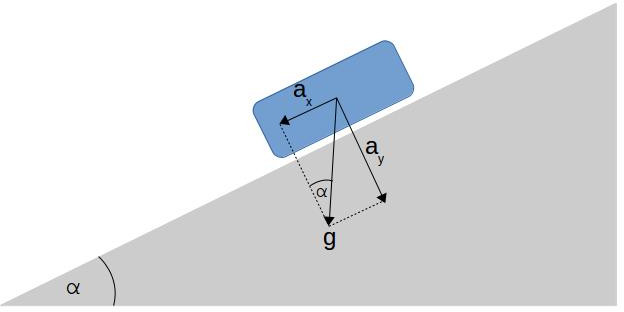
\includegraphics[scale=0.5]{katNachylenia.jpg}
    \caption{Równia pochyła - przykład ilustrujący sposób wyznaczenia kąta nachylenia terenu.}
    \label{fig:rownia}
\end{figure}
%____________________________________________________________________________________________________________ 
\subsection{Analiza danych pomiarowych żyroskopu}
\label{gyro}
Zgodnie z zależnością (\ref{eq:predkoscKatowa}) prędkość kątowa określana jest jako zmiana drogi kątowej w czasie. Sytuacja odwrotna, czyli wyznaczenie drogi kątowej na podstawie pomiarów prędkości kątowej polega na znalezieniu funkcji odwrotnej:
\begin{equation}  
    \alpha = \int{\omega_{z}(t)dt}
    \label{eq:zyroRad}
\end{equation}
gdzie:
\begin{eqwhere}[2cm]
	\item[$\omega_{z}(t)$] prędkość kątowa wzdłuż osi $Z$ żyroskopu.
	
\end{eqwhere}

Podobnie, jak zależność (\ref{eq:rowniaRadian}), równanie (\ref{eq:zyroRad}) pozwala wyznaczyć miarę łukową wyrażoną w radianach.

Operacja całkowania prędkości kątowej została uwzględniona w projekcie filtru komplementarnego w postaci dodatkowego członu całkującego, którego transmitancja operatorowa wynosi $\frac{1}{s}$ - wzór (\ref{eq:alpha}) w pkt. \ref{kompZasadaDzialania}.

%____________________________________________________________________________________________________________ 
\subsection{Filtr komplementarny}
\label{kompZasadaDzialania}
Zasada działania filtru komplementarnego polega na odpowiedniej fuzji danych pochodzących z różnych czujników pomiarowych. Sygnał każdego z nich zawiera istotną informację o mierzonej wielkości jak również zakłócenia, które powinny zostać wyeliminowane. Fuzja danych polega na zastosowaniu odpowiednich filtrów, dolnoprzepustowych, środkowoprzepustowych i górnoprzepustowych, które eliminują zakłócenia charakterystyczne dla danego czujnika, jednocześnie przenosząc informacje użyteczne. Warunkiem koniecznym uzyskania dokładniejszych wartości estymowanych, od wartości mierzonych, jest zastosowanie czujników pomiarowych o różnej charakterystyce częstotliwości błędów pomiarowych. Schemat przedstawiający ogólną idę filtru komplementarnego zamieszczono na rys \ref{fig:kompGeneral}.
\begin{figure}[h]
    \centering
    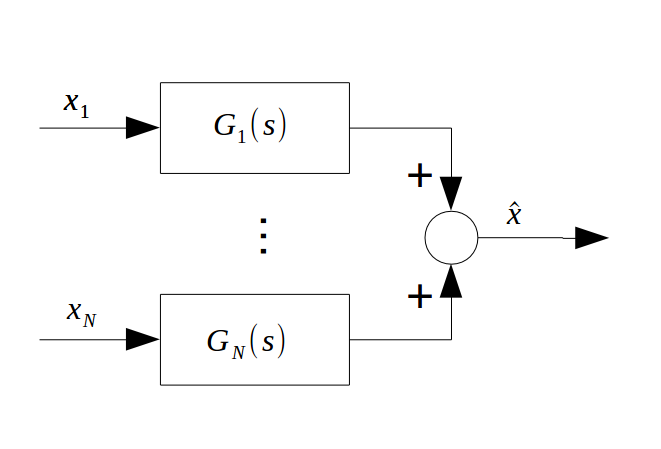
\includegraphics[scale=0.3]{filtrKomp.png}
    \caption{Zasada działania filtru komplementarnego. $x_1$ : $x_N$ - sygnały wejściowe, $G_1(s) : G_N(s)$ - transmitancje operatorowe poszczególnych filtrów, $\hat{x}$ - estymowana wartość wyjściowa.}
    \label{fig:kompGeneral}
\end{figure}

Zaprojektowany filtr nie powinien wprowadzać dodatkowej dynamiki - transmitancja operatorowa, określająca stosunek transformaty Laplace'a sygnału wyjściowego do transformaty Laplace'a sygnału wejściowego, powinna spełniać zależność \cite{komplementarny}:
\begin{equation}
    G(s)=\sum_{i=1}^{N}G_{i}(s)=1
    \label{eq:zasadaKomplementarnosci}
\end{equation}

W odniesieniu do estymacji wartości kąta nachylenia podłoża, schemat filtru komplementarnego, wykorzystującego wartości kątów wyznaczonych na podstawie danych pomiarowych pochodzących z akcelerometru oraz żyroskopu, przedstawiony został na rys \ref{fig:kompKat}. 

\begin{figure}[h]
    \centering
    \includegraphics[scale=0.34]{tests_akcelerometrBezRuchu.jpg}
    \caption{Kąt nachylenia podłoża wyznaczony na podstawie pomiaru składowych przyspieszenia ziemskiego, akcelerometr pozostaje w spoczynku.}
    \label{fig:tests_akcelerometrBezRuchu}
\end{figure}

Pomiar składowych przyspieszenia ziemskiego umożliwia wyznaczenie kąta nachylenia podłoża (pkt. \ref{pomiaryAkcel}). Ta metoda znajduje swoje zastosowanie wtedy, gdy układ pomiarowy nie porusza się lub porusza się ruchem jednostajnym. Na rysunku \ref{fig:tests_akcelerometrBezRuchu} przedstawiono przebieg wartości kąta nachylenia, gdy akcelerometr pozostaje w spoczynku a kąt nachylenia wynosi 0$^{\circ}$. Zaobserwowano minimalne chwilowe odchyłki wartości kąta nachylenia.

W ruchu przyspieszonym dane pomiarowe akcelerometru uwzględniają siły powodujące ten ruch, a brak możliwości odseparowania składowych przyspieszenia ziemskiego sprawia, że kąt nachylenia obarczony jest błędem. Należy zatem zastosować filtr dolnoprzepustowy, eliminujący szybkozmienne wartości kąta nachylenia pochodzące z akcelerometru. Na rysunku \ref{fig:akcelerometrRuch} przedstawiono przebieg wartości kąta nachylenia, gdy akcelerometr poruszał się ruchem posuwisto-zwrotnym po płaskiej powierzchni. Kąt nachylenia nie ulega zmianie, jednak ze względu na siły, zakłócające pomiar przyspieszenia ziemskiego, można zaobserwować bardzo duże błędy wartości kąta nachylenia podłoża, osiągające nawet 20$^{\circ}$.

\begin{figure}[h]
    \centering
    \includegraphics[scale=0.34]{tests_akcelerometrRuch.jpg}
    \caption{Kąt nachylenia podłoża wyznaczony na podstawie pomiaru składowych przyspieszenia ziemskiego, akcelerometr porusza się ruchem posuwisto-zwrotnym.}
    \label{fig:akcelerometrRuch}
\end{figure}

Żyroskop służy do pomiaru prędkości obrotowej. Całkowanie prędkości obrotowej umożliwia wyznaczenie kąta nachylenia podłoża (pkt. \ref{gyro}). Jednak zakłócenia toru pomiarowego oraz wrażliwość na warunki pracy, a w szczególności temperaturę, powodują zjawisko tzw. dryfu żyroskopowego, przedstawionego na rys. \ref{fig:tests_dryft}. Dryf spowodowany jest ciągłym narastaniem błędów, w wyniku całkowania zakłóconych danych pomiarowych. Można zaobserwować, że na rys. \ref{fig:tests_dryft} wartość kąta nachylenia podłoża rośnie, pomimo iż żyroskop pozostaje w spoczynku a kąt nachylenia nie ulega zmianie. Błędy powstałe w wyniku dryfu żyroskopowego są sygnałami wolnozmiennymi. Zastosowanie filtru górnoprzepustowego pozwala je wyeliminować.
\begin{figure}[h]
    \centering
    \includegraphics[scale=0.34]{tests_dryft.jpg}
    \caption{Zjawisko dryfu żyroskopu.}
    \label{fig:tests_dryft}
\end{figure}

Filtr dolnoprzepustowy może zostać zrealizowany poprzez obiekt inercyjny I rzędu(pkt. \ref{filtrRc}):
\begin{equation}
    G_{low}(s)=\frac{1}{Ts+1}
    \label{eq:lowPass}
\end{equation}

Zgodnie z równaniem (\ref{eq:zasadaKomplementarnosci}), filtr górnoprzepustowy powinien spełniać zależność:
\begin{equation}
    G_{high}(s)=1-G_{1}(s)=\frac{Ts}{Ts+1}
    \label{eq:highPass}
\end{equation}

Transmitancja $G_{high}(s)$ odpowiada transmitancji filtru górnoprzepustowego RC.

\begin{figure}[h]
    \centering
    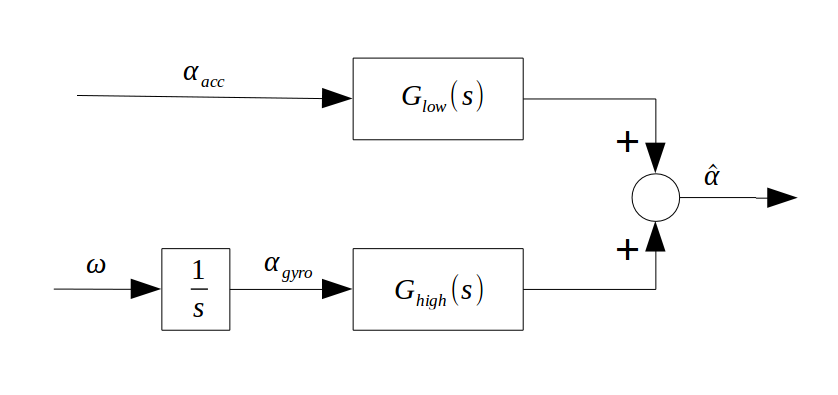
\includegraphics[scale=0.34]{filtrKompKat.png}
    \caption{Schemat filtru komplementarnego estymującego wartość kąta nachylenia podłoża.}
    \label{fig:kompKat}
\end{figure}

Estymowana wartość kąta nachylenia $\hat{\alpha}$ spełnia zależność:
\begin{equation}
    \hat{\alpha} = \frac{1}{Ts+1}\alpha_{acc}+\frac{Ts}{Ts+1}\frac{1}{s}\omega = \frac{\alpha_{acc}+T\omega}{Ts + 1}
    \label{eq:alpha}
\end{equation}
gdzie:
\begin{eqwhere}[2cm]
	\item[$\hat{\alpha}$] estymowana wartość kąta nachylenia,
	\item[$\alpha_{acc}$] kąt nachylania wyznaczony na podstawie danych z akcelerometru,
	\item[$\omega$] prędkość obrotowa.
\end{eqwhere}

Ze względu na potrzebę zaimplementowania filtru w układzie mikroprocesorowym, należy znaleźć równoważny model dyskretny, który aproksymuje własności dynamiczne modelu ciągłego. Można tego dokonać stosując metodę Eulera wstecz \cite{grega}:
\begin{equation}
    s=\frac{t_0z}{z-1}
    \label{eq:eulerWstecz}
\end{equation}
gdzie:
\begin{eqwhere}[2cm]
	\item[$t_{0}$] długość kroku dyskretyzacji.
\end{eqwhere}

Podstawiając zależność (\ref{eq:eulerWstecz}) do równania (\ref{eq:alpha}) oraz przyjmując podstawienie $p = \frac{T}{T + t_0}$, gdzie $T$ to stała czasowa filtru,  równanie różnicowe estymujące wartość kąta nachylania podłoża przyjmuje postać:
\begin{equation}
    \hat{\alpha_{k}} = p(\hat{\alpha}_{k-1} + \omega_{k}t_0) + (1-p)\alpha_{acc}
\end{equation}


% itd.
% \appendix
% \include{dodatekA}
% \include{dodatekB}
% itd.
\printbibliography

\end{document}
